\chapter{Operations on stable functions}
\label{chap:operations}

Having identified several classes of stable generalized density functions (GDFs)
in Chapter~\ref{chap:stable_functions}, we now turn to natural subsequent
questions: \emph{how does stability behave under common operations?
If we combine stable GDFs, for instance, by addition or by taking their minimum,
is the resulting GDF also stable? If so, can we bound its stability constant in
terms of the constants of the original functions?}
This chapter explores these questions, identifying conditions under which
stability is preserved and providing counterexamples where it is not.
Understanding these properties is crucial for constructing more complex stable
GDFs from simpler ones and for gaining deeper insight into the structure of the
space of stable functions.

\section{Affine transformations}

We begin with the simplest operations: adding a constant to a stable GDF and
multiplying it by a constant.

\begin{theorem}[Stability under constant addition]
    \label{thm:constant_addition}
    Let $f(P, x)$ be a $c$-stable GDF with $q$-tame induced persistence modules.
    Then for any constant $z \in \mathbb{R}$ the GDF
    $g(P, x) = f(P, x) + z$ is also $c$-stable with $q$-tame induced
    persistence modules.
\end{theorem}
\begin{proof}
    \begin{figure}
        \centering
        \pgfmathsetmacro{\off}{6.5}
        \pgfmathsetmacro{\z}{1.3}
        \hspace*{-1cm}
        \begin{tikzpicture}
            \small
            % Axes
            \draw[->] (0,0) -- (5,0) node[right] {Birth};
            \draw[->] (0,0) -- (0,5.5) node[above] {Death};
            \draw[->] ({\off},0) -- ({6+\off},0) node[right] {Birth};
            \draw[->] ({\off},0) -- ({\off},5.5) node[above] {Death};
            
            % Grid
            % \draw[gray!30] (0,0) grid (6,6);
            
            % Diagonal
            \draw[dashed] (0,0) -- (5,5);
            \draw[dashed] ({\off},0) -- ({5+\off},5);
            
            % Point coords
            \coordinate (p1) at (1.3,3);
            \coordinate (p1z) at ($(p1) + (\z,\z)$);
            \coordinate (p2) at (0.8,1.3);
            \coordinate (p2z) at ($(p2) + (\z,\z)$);
            \coordinate (p3) at (3,5);
            \coordinate (p3z) at ($(p3) + (\z,0)$);
            
            \coordinate (q1) at ({\off + 1.1},2.6);
            \coordinate (q1z) at ($(q1) + (\z,\z)$);
            \coordinate (q2) at ({\off + 1},1);
            \coordinate (q2z) at ($(q2) + (\z,\z)$);
            \coordinate (q3) at ({\off + 2.5},5);
            \coordinate (q3z) at ($(q3) + (\z,0)$);
            
            % Lines to axes
            % \draw[dashed,gray] (p1) -- (p1 |- 0,0) node[below,blue,rotate=45,anchor=east] {$b_1$};
            % \draw[dashed,gray] (p1) -- (0,0 |- p1) node[left,blue] {$d_1$};
            % \draw[dashed,gray] (p1z) -- (p1z |- 0,0) node[below,red,rotate=45,anchor=east] {$b_1+z$};
            % \draw[dashed,gray] (p1z) -- (0,0 |- p1z) node[left,red] {$d_1+z$};
            % \draw[dashed,gray] (p2) -- (p2 |- 0,0) node[below,blue,rotate=45,anchor=east] {$b_2$};
            % \draw[dashed,gray] (p2) -- (0,0 |- p2) node[left,blue] {$d_2$};
            % \draw[dashed,gray] (p2z) -- (p2z |- 0,0) node[below,red,rotate=45,anchor=east] {$b_2+z$};
            % \draw[dashed,gray] (p2z) -- (0,0 |- p2z) node[left,red] {$d_2+z$};
            % \draw[dashed,gray] (p3) -- (p3 |- 0,0) node[below,blue,rotate=45,anchor=east] {$b_3$};
            % \draw[dashed,gray] (p3z) -- (p3z |- 0,0) node[below,red,rotate=45,anchor=east] {$b_3+z$};
            % \draw[dashed,gray] (5,5) -- (0,5) node[left,black] {$\infty$};

            % Points
            \fill[blue] (p1) circle (2pt) node[above left,blue] {$p_1$};
            \fill[blue] (p2) circle (2pt) node[above left,blue] {$p_2$};
            \fill[blue] (p3) circle (2pt) node[above left,blue] {$p_3$};
            \fill[red] (p1z) circle (2pt) node[above left,red] {$p_1+z$};
            \fill[red] (p2z) circle (2pt) node[above right,red] {$p_2+z$};
            \fill[red] (p3z) circle (2pt) node[above left,red] {$p_3+z$};

            \fill[blue] (q1) circle (2pt) node[above right,blue] {$q_1$};
            \fill[blue] (q2) circle (2pt) node[below right,blue] {$q_2$};
            \fill[blue] (q3) circle (2pt) node[above left,blue] {$q_3$};
            \fill[red] (q1z) circle (2pt) node[above right,red] {$q_1+z$};
            \fill[red] (q2z) circle (2pt) node[below right,red] {$q_2+z$};
            \fill[red] (q3z) circle (2pt) node[above right,red] {$q_3+z$};
            
            \path[blue, bend left=10, shorten <= 0.15cm, shorten >= 0.15cm] (p1) edge (q1);
            \path[blue, bend right=20, shorten <= 0.15cm, shorten >= 0.15cm] (p2) edge (q2);
            \path[blue, bend right, shorten <= 0.15cm, shorten >= 0.15cm] (p3) edge (q3);
            \path[red, bend right=10, shorten <= 0.15cm, shorten >= 0.15cm] (p1z) edge (q1z);
            \path[red, bend right=20, shorten <= 0.15cm, shorten >= 0.15cm] (p2z) edge (q2z);
            \path[red, bend left, shorten <= 0.15cm, shorten >= 0.15cm] (p3z) edge (q3z);
        \end{tikzpicture}
        \caption{
            The persistence diagrams of $f_P$ (left, blue), $f_Q$ (right, blue),
            and $g_P$ (left, red), $g_Q$ (right, red) where $g_P = f_P + z$ and
            $g_Q = f_Q + z$. A matching between the diagrams of $f_P$ and
            $f_Q$ is shown in blue, and a matching between the diagrams of
            $g_P$ and $g_Q$ is shown in red.
        }
        \label{fig:constant_addition_pds}
    \end{figure}

    First we relate the sublevel sets of $g_P$ and $f_P$.
    For any $a \in \R$:
    \begin{align}
        g^{-1}_P(-\infty, a] &= \{x \in \R^d \mid g_P(x) \leq a\} \\
        &= \{x \in \R^d \mid f_P(x) + z \leq a\} \\
        &= \{x \in \R^d \mid f_P(x) \leq a - z\} \\
        &= f^{-1}_P(-\infty, a - z].
    \end{align}
    This means the sublevel set filtration $\{g_P^{-1}(-\infty, a]\}_{a\in \R}$
    is identical to the filtration $\{f_P^{-1}(-\infty, b]\}_{b\in \R}$ but
    with the indices shifted by $z$, i.e., $b = a - z$.
    Consequently, if a topological feature is born at $b$ and dies at $d$ in
    the filtration of $f_P$, a corresponding feature of the same dimensionality
    in the filtration of $g_P$ will be born at $b + z$ and die at $d + z$, and
    vice versa.
    Thus, the persistence diagrams of $f_P$ and $g_P$ are related by a constant
    shift along both axes:
    \begin{equation}
        \dgm_k(g_P) = \{(b + z, d + z) \mid (b, d) \in \dgm_k(f_P)\}.
    \end{equation}
    
    Next, we address $q$-tameness.
    Let $\mathbb{F} = (\{F_a\}, \{\mathfrak{f}_a^{a'}\})$ be a persistence
    module induced by $f_P$ and
    $\mathbb{G} = (\{G_a\}, \{\mathfrak{g}_a^{a'}\})$ be that induced by $g_P$.
    From the relationship between the sublevel sets, we have
    $G_a = F_{a - z}$ and $\mathfrak{g}_a^{a'} = \mathfrak{f}_{a - z}^{a' - z}$.
    Since $\mathbb{F}$ is $q$-tame by assumption, $\mathfrak{f}_a^{a'}$ is of
    finite rank for $a < a'$.
    This directly implies that $\mathfrak{g}_a^{a'}$ is also of finite rank for
    all $a < a'$, so $\mathbb{G}$ is also $q$-tame.
    
    Finally, we prove $c$-stability for $g$.
    Fix point clouds $P$ and $Q$.
    By stability of $f$, we have that
    \begin{equation}
        d_b(\dgm_k(f_P), \dgm_k(f_Q)) \leq c \cdot d_H(P, Q).
    \end{equation}
    Let $\pi_i$ be a sequence of matchings between $\dgm_k(f_P) \cup \Delta$ and
    $\dgm_k(f_Q) \cup \Delta$ that achieves this bound.
    For each $i$, we can construct a matching $\pi'_i$ between
    $\dgm_k(g_P) \cup \Delta$ and $\dgm_k(g_Q) \cup \Delta$ by shifting the
    points in $\pi_i$ by $z$:
    \begin{equation}
        \pi'_i(b + z, d + z) = (b' + z, d' + z) \text{ where } (b', d') = \pi_i(b, d).
    \end{equation}
    The cost of this matching is the same as that of $\pi_i$:
    \begin{equation}
        \norm{(b + z, d + z) - \pi'_i(b + z, d + z)}_\infty = \norm{(b, d) - (b', d')}_\infty,
    \end{equation}
    thus $\pi_i'$ is a matching between $\dgm_k(g_P)$ and $\dgm_k(g_Q)$ with the same
    cost as $\pi_i$. An example of this is shown in
    Figure~\ref{fig:constant_addition_pds}.
    Therefore, we have:
    \begin{equation}
        d_b(\dgm_k(g_P), \dgm_k(g_Q)) \leq c \cdot d_H(P, Q).
    \end{equation}
    Since this holds for arbitrary $P$ and $Q$, $g$ is $c$-stable.
\end{proof}

\begin{theorem}[Stability under positive constant multiplication]
    \label{thm:constant_nonneg_multiplication}
    Let $f(P, x)$ be a $c$-stable GDF with $q$-tame induced persistence modules.
    Then for any constant $\alpha \geq 0$, the function
    $g(P, x) = \alpha f(P, x)$ is a $(c\alpha)$-stable GDF with $q$-tame induced
    persistence modules.
\end{theorem}
\begin{proof}
    We first consider the case when $\alpha = 0$.
    In this case, $g(P, x) = 0$ for all $x \in \R^d$, which is $0$-stable
    by Theorem~\ref{thm:independent_stable}. Its induced persistence modules
    are pointwise finite dimensional, hence $q$-tame.
    
    Now, let $\alpha > 0$.
    The argument mirrors that of Theorem~\ref{thm:constant_addition}.
    The sublevel sets of $g$ and of $f$ are related by:
    \begin{equation}
        g^{-1}_P(-\infty, a] = \{x \in \R^d \mid \alpha f_P(x) \leq a\} = f^{-1}_P(-\infty, a/\alpha].
    \end{equation}
    This implies that the persistence module $\mathbb{G}$ induced by $g_P$ is
    the same as the persistence module $\mathbb{F}$ induced by $f_P$ up to reindexing where $a$ is replaced with $a \cdot \alpha$, i.e.
    $F_a = G_{a \cdot \alpha}$ and the maps $\mathfrak{f}_a^{a'}$ and
    $\mathfrak{g}_{\alpha \cdot a}^{\alpha \cdot a'}$ are identical.
    The $q$-tameness of $\mathbb{F}$ implies the $q$-tameness of $\mathbb{G}$.

    A point $(b, d)\in \dgm_k(f_P)$ corresponds to $(\alpha b, \alpha d) \in
    \dgm_k(g_P)$ and vice versa. By the same argument as in the proof of
    Theorem~\ref{thm:constant_addition}, we can construct a matching
    $\pi'_i(b \cdot \alpha, d \cdot \alpha) = (b' \cdot \alpha, d' \cdot \alpha)$ where
    $(b', d') = \pi_i(b, d)$, which gives a bound on the bottleneck distance
    between the persistence diagrams of $g_P$ and $g_Q$:
    \begin{equation}
        d_b(\dgm_k(g_P), \dgm_k(g_Q)) \leq c \cdot \alpha \cdot d_H(P, Q).
    \end{equation}
\end{proof}

We can extend this theorem to negative constants using the following lemma:
\begin{lemma}[Stability under negation]
    \label{lem:negation_stability}
    Let $f(P, x)$ be a $c$-stable GDF with $q$-tame induced persistence modules.
    Then the function $g(P, x) = - f(P, x)$ is also a $c$-stable GDF
    with $q$-tame induced persistence modules.
\end{lemma}
\begin{proof}
    This result follows directly from the symmetry theorem by David Cohen-Steiner,
    Herbert Edelsbrunner, and John Harer~\cite{cohen2009extending}.
    The theorem states that for any real-valued function $f$ on a
    $d$-dimensional manifold, the persistence diagram of $f$ in dimension $k$
    is related to the persistence diagram of $-f$ in dimension $d - k$ via
    reflection across the minor diagonal (the line $b + d = 0$).
    More precisely, for every point $(b, d) \in \dgm_k(f)$, there corresponds a point
    $(-d, -b) \in \dgm_{d - k}(-f)$, and this correspondence is bijective.

    Given that $\R^d$ is a $d$-manifold, we can apply this theorem.
    Now let $P, Q \in \mathcal{P}(\R^d)$ be finite point clouds and $f$ be a
    $c$-stable GDF with $q$-tame induced persistence modules.
    Let the bottleneck distance $d_b(\dgm_k(f_P), \dgm_k(f_Q))$ be achieved
    by a sequence of matchings $\pi_i$ between the diagrams.
    We can construct a sequence of matchings $\pi'_i$ between the diagrams
    $\dgm_{d - k}(f_P)$ and $\dgm_{d - k}(f_Q)$ by reflecting the points
    in $\pi_i$ across the minor diagonal:
    \begin{equation}
        \pi'_i(-d, -b) = (-d', -b') \text{ where } \pi_i(b, d') = (b', d').
    \end{equation}
    By the symmetry theorem, this is a valid sequence of matchings and the cost
    of $\pi'_i$ is the same as that of $\pi_i$, thus $-f$ is also $c$-stable.
    
    $q$-tameness follows from the fact that the induced persistence modules
    of $f$ and $-f$ are identical up to reindexing with the sign change.
\end{proof}

Combining Theorem~\ref{thm:constant_nonneg_multiplication} and
Lemma~\ref{lem:negation_stability}, we obtain the following corollary:
\begin{corollary}[Stability under constant multiplication]
    \label{cor:constant_multiplication}
    Let $f(P, x)$ be a $c$-stable GDF with $q$-tame induced persistence modules.
    Then for any constant $\alpha \in \mathbb{R}$, the function
    $g(P, x) = \alpha f(P, x)$ is also a $c|\alpha|$-stable GDF with
    $q$-tame induced persistence modules.
\end{corollary}

\section{Addition of stable functions}
\label{sec:addition_stable}

Having examined affine transformations, we now explore the effect of adding two
stable GDFs.
Let $f$ and $g$ be GDFs with stability constants $c_f$ and $c_g$.
What can be said about the stability constant of their sum
$h(P, x) = f(P, x) + g(P, x)$?
A simple case offers initial intuition:
if $g = f$, then $h = f + f = 2 \cdot f$.
By Theorem~\ref{thm:constant_addition}, $h$ is $(2 \cdot c_f)$-stable.
One would naturally expect that the stability constant of
$h = f + g$ is then bounded by $c_f + c_g$, but this is not always the case,
as the following example demonstrates.
\begin{example}[Sum of stable GDFs may not be stable]
    Consider GDFs on $\R$ ($d = 1$).
    Fix a constant $a > 0$, let
    \begin{equation}
        f(P, x) = x + a \cdot \min P \quad \text{and} \quad g(P, x) = - x + a \cdot \min P.
    \end{equation}
    As described in Example~\ref{ex:x_plus_g}, both GDFs are $0$-stable.

    The sum of $f$ and $g$ is:
    \begin{equation}
        h(P, x) = f(P, x) + g(P, x) = 2a \cdot \min P.
    \end{equation}
    The function $h_P$ is constant for a fixed $P$.
    Its 0-dimensional persistence diagram has exactly one point
    $(2a \cdot \min P, \infty)$, representing the single connected component
    $\R$ itself, born at $2a \cdot \min P$ and never dying, as can be seen
    in Figure~\ref{fig:sum_stable_gdfs}.
    
    \begin{figure}
        \centering
        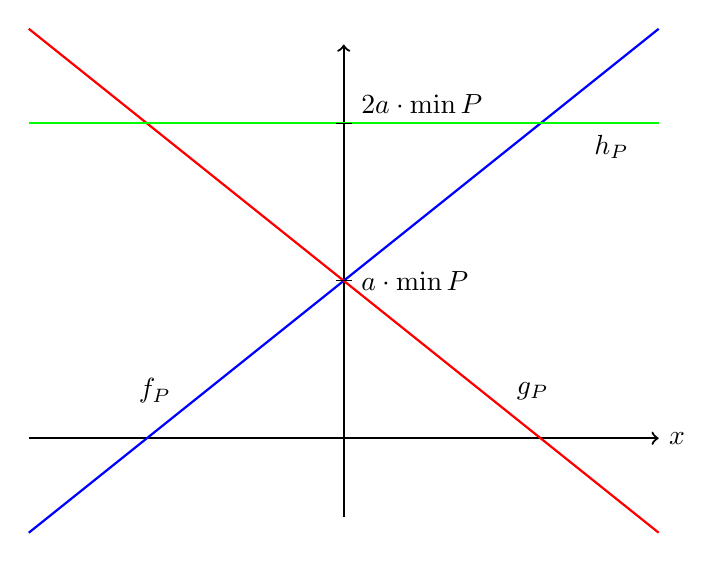
\begin{tikzpicture}[scale=2]
            % Axes
            \draw[thick, ->] (-2,0) -- (2,0) node[right] {$x$};
            \draw[thick, ->] (0,-0.5) -- (0,2.5);

            \draw[domain=-2:2, smooth, variable=\x, blue, thick] plot ({\x}, {0.8*\x+1});
            \draw[domain=-2:2, smooth, variable=\x, red, thick] plot ({\x}, {-0.8*\x+1});
            \draw[domain=-2:2, smooth, variable=\x, green, thick] plot ({\x}, {2});

            \draw (-0.05, 1) -- (0.05, 1);
            \node[right] at (0.05, 1) {$a \cdot \min P$};
            \draw (-0.05, 2) -- (0.05, 2);
            \node[above right] at (0.05, 2) {$2a \cdot \min P$};

            \node at (1.2, 0.3) {$g_P$};
            \node at (-1.2, 0.3) {$f_P$};
            \node at (1.7, 1.85) {$h_P$};
        \end{tikzpicture}
        \caption{The GDFs $f_P$ (red), $g_P$ (blue) and $h_P$ (green) for
            an arbitrary point cloud $P$.}
        \label{fig:sum_stable_gdfs}
    \end{figure}
    
    Let $P = \{1\}, Q = \{2\}$ with $d_H(P, Q) = 1$.
    The 0-dimensional persistence diagrams of $h$ are
    $\dgm_0(h_P) = \{(2a, \infty)\}$ and $\dgm_0(h_Q) = \{(4a, \infty)\}$.
    In the optimal matching $\pi$ between these diagrams, the point $(2a, \infty)$
    must be matched to $(4a, \infty)$, as matching either of them to the
    diagonal $\Delta$ would result in an infinite cost.
    The cost of $\pi$ is thus:
    \begin{equation}
        \norm{(2a, \infty) - (4a, \infty)}_\infty = 2a.
    \end{equation}
    Therefore, the bottleneck distance between the diagrams is $2a$,
    and for $h$ to be $c$-stable, we need:
    \begin{equation}
        2a \leq c \cdot d_H(P, Q) = c.
    \end{equation}
    This means that for any $c \in [0, \infty)$, we can choose $a = c$ such that
    the stability constant of $h$ is larger than $c$.
    Thus, the sum of two $0$-stable GDFs is not necessarily $c$-stable for
    any $c \in [0, \infty)$.
\end{example}

Despite this counterexample for general stable GDFs, stability under addition
holds for the more restrictive class of PC-Lipschitz GDFs.
\begin{theorem}[Sum of PC-Lipschitz GDFs]
    \label{thm:sum_pc_lipschitz}
    Let $f(P, x)$ and $g(P, x)$ be a $c_f$-PC-Lipschitz GDF and a
    $c_g$-PC-Lipschitz GDF. Then their sum $h(P, x) = f(P, x) + g(P, x)$ is
    a $(c_f + c_g)$-PC-Lipschitz GDF and is thus $(c_f + c_g)$-stable
    if the induced persistence modules of $h$ are $q$-tame.
\end{theorem}
\begin{proof}
    Let $P, Q \subseteq \R^d$ be finite point clouds.
    By subadditivity of the $\infty$-norm and the definition of
    PC-Lipschitz continuity, we have:
    \begin{align}
        \norm{h_P - h_Q}_\infty &= \norm{(f_P + g_P) - (f_Q + g_Q)}_\infty \\
        & \leq \norm{f_P - f_Q}_\infty + \norm{g_P - g_Q}_\infty \\
        & \leq c_f \cdot d_H(P, Q) + c_g \cdot d_H(P, Q) \\
        & = (c_f + c_g) \cdot d_H(P, Q),
    \end{align}
    which shows that $h$ is ($c_f + c_g$)PC-Lipschitz.
    By Lemma~\ref{lem:pc_lipschitz_stable}, $h$ is $(c_f + c_g)$-stable if its
    induced persistence modules are $q$-tame.
\end{proof}

\section{Minimum and maximum of stable functions}

Similar to addition, the pointwise minimum of two PC-Lipschitz GDFs is also
PC-Lipschitz, and thus stable.
\begin{theorem}[Minimum of PC-Lipschitz GDFs]
    \label{thm:min_pc_lipschitz}
    Let $f(P, x)$ and $g(P, x)$ be a $c_f$-PC-Lipschitz GDF and a
    $c_g$-PC-Lipschitz GDF.
    Then the function $h(P, x) = \min\{f(P, x), g(P, x)\}$
    is a $\max\{c_f, c_g\}$-PC-Lipschitz GDF and is thus $\max\{c_f, c_g\}$-stable
    if the induced persistence modules of $h$ are $q$-tame.
\end{theorem}
\begin{proof}
    This result follows directly from a standard property of Lipschitz
    functions: the pointwise minimum (or maximum) of two Lipschitz functions
    $F_1, F_2: X \to Y$ with Lipschitz constants $L_1, L_2$ is itself
    Lipschitz with constant $\max\{L_1, L_2\}$~(\cite{weaver2018lipschitz},
    Proposition~1.5.5).
\end{proof}

However, this property does not hold for general stable GDFs, as shown in the
following counterexample.
\begin{example}[Minimum of $0$-stable GDFs can be unstable]
    \begin{figure}
        \centering
        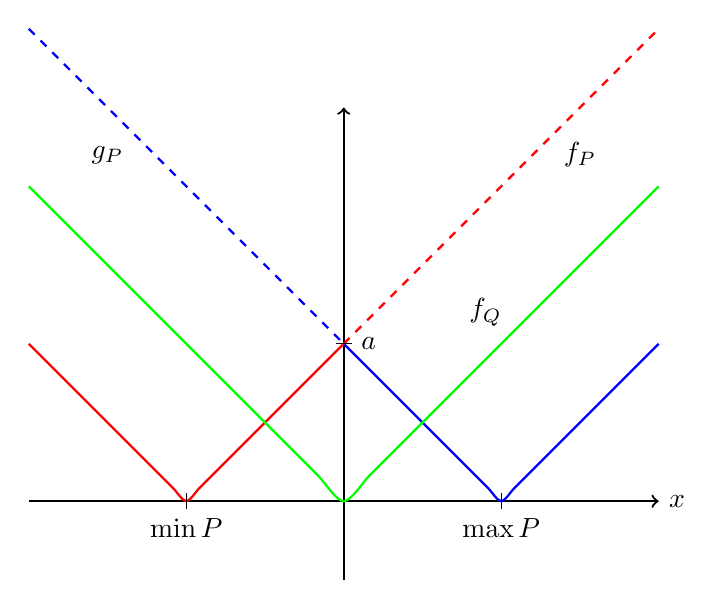
\begin{tikzpicture}[scale=2]
            % Axes
            \draw[thick, ->] (-2,0) -- (2,0) node[right] {$x$};
            \draw[thick, ->] (0,-0.5) -- (0,2.5);

            \draw[domain=-2:0, smooth, dashed, variable=\x, blue, thick] plot ({\x}, {abs(\x-1)});
            \draw[domain=0:2, smooth, dashed, variable=\x, red, thick] plot ({\x}, {abs(\x+1)});
            \draw[domain=0:2, smooth, variable=\x, blue, thick] plot ({\x}, {abs(\x-1)});
            \draw[domain=-2:0, smooth, variable=\x, red, thick] plot ({\x}, {abs(\x+1)});
            \draw[domain=-2:2, smooth, variable=\x, green, thick] plot ({\x}, {abs(\x)});

            % Indicate minima points
            \node[below] at (-1,-0.05) {$\min P$};
            \draw (-1, -0.05) -- (-1, 0.05);

            \node[below] at (1,-0.05) {$\max P$};
            \draw (1, -0.05) -- (1, 0.05);
            
            \draw (-0.05, 1) -- (0.05, 1);
            \node[right] at (0.05, 1) {$a$};
            \node at (-1.5, 2.2) {$g_P$};
            \node at (1.5, 2.2) {$f_P$};
            \node at (0.9, 1.2) {$f_Q$};
        \end{tikzpicture}
        \caption{The GDFs $f_P$ (red), $g_P$ (blue) and $f_Q$ (green) for
            point clouds $P = \{-1, 1\}$ and $Q = \{0\}$.
            The minimum $h_P$ of $f_P$ and $g_P$ is shown in solid red and green
            lines.}
        \label{fig:min_max_stable_gdfs}
    \end{figure}

    Consider GDFs on $\R$ ($d = 1$).
    Fix a constant $a \in \R$ and let
    \begin{equation}
        f(P, x) = a \cdot |x - \min p| \quad \text{and} \quad g(P, x) = a \cdot |x - \max p|.
    \end{equation}
    The 0-dimensional persistence diagrams for these GDFs are
    $\dgm_0(f_P) = \{(0, \infty)\}$ and $\dgm_0(g_P) = \{(0, \infty)\}$ for any
    $P$, and thus are both $0$-stable.

    Consider $P = \{-1, 1\}$ and $Q = \{0\}$ with $d_H(P, Q) = 1$.
    As we can see in Figure~\ref{fig:min_max_stable_gdfs}, the 0-dimensional
    persistence diagrams of $h_P$ and $h_Q$ are
    \begin{align}
        \dgm_0(h_P) &= \{(0, a), (0, \infty)\}, \\
        \dgm_0(h_Q) &= \{(0, \infty)\}.
    \end{align}
    The cost of matching $(0, a)$ to $\Delta$ is $\frac{a}{2}$, so the
    bottleneck distance between the diagrams is $\frac{a}{2}$.
    Thus, for every $c \in [0, \infty)$ we can choose $a = 2c$ such that
    the stability constant of $h(P, x) = f(P, x) + g(P, x)$ is $c$.
    Thus, the minimum of two $0$-stable GDFs is not necessarily
    $c$-stable for any $c \in [0, \infty)$.
\end{example}

This example shows that stability alone is not sufficient to guarantee that the
minimum of two GDFs is stable. The issue arose because the topological changes
induced by perturbing the point cloud were different for the two functions,
leading to an unstable interaction in their minimum. This suggests that for
stability to be preserved, the interleaving maps of the two functions must be
compatible. Building on this intuition, we can establish conditions for
stability that are not reliant on the strong PC-Lipschitz property.

\begin{theorem}
    Let $f$ and $g$ be $c_f$-stable and $c_g$-stable GDFs, respectively.
    Let the sublevel sets of $f$ and $g$ be denoted as
    $f(P)_a = f^{-1}_P(-\infty, a]$ and $g(P)_a = g^{-1}_P(-\infty, a]$.

    Assume that for any finite point clouds $P, Q \in \mathcal{P}(X)$:
    \begin{enumerate}
        \item The induced persistence modules $\mathbb{F}_P$ and $\mathbb{G}_P$
        are $q$-tame.
        \item The functions $f_P, g_P$ are continuous.
        \item The stability of $f$ and $g$ is realised by interleavings of their
        sublevel set filtrations, i.e.:
        \begin{align}
            c_f \cdot d_H(P, Q) = d_i(\mathbb{F}_P, \mathbb{F}_Q) &= d_i(\{f(P)_a\}, \{f(Q)_a\}) \\
            c_g \cdot d_H(P, Q) = d_i(\mathbb{G}_P, \mathbb{G}_Q) &= d_i(\{g(P)_a\}, \{g(Q)_a\}).
        \end{align}
        Let these interleavings be realised by maps
        \begin{align}
            \varphi^f_a & : f(P)_a \to f(Q)_{a + c_f \cdot d_H(P, Q)} \\
            \psi^f_a & : f(Q)_a \to f(P)_{a + c_f \cdot d_H(P, Q)} \\
            \varphi^g_a & : g(P)_a \to g(Q)_{a + c_g \cdot d_H(P, Q)} \\
            \psi^g_a & : g(Q)_a \to g(P)_{a + c_g \cdot d_H(P, Q)}.
        \end{align}
        \item \label{item:min_agree} For all $x \in \R^d$ such that $f(P, x) =
        g(P, x)$, we also have that $\varphi_a^f(x) = \varphi_a^g(x)$ and
        $\psi_a^f(x) = \psi_a^g(x)$.
        \item \label{item:min_monotone} For all $x \in \R^d$ such that $f(P, x)
        \leq g(P, x)$, we also have that $f(Q, x) \leq g(Q, x)$.
    \end{enumerate}
    Then the function $h(P, x) = \min\{f(P, x), g(P, x)\}$ is
    a $\max\{c_f, c_g\}$-stable GDF if the induced persistence modules of $h$
    are $q$-tame.
\end{theorem}
\begin{proof}
    Fix $P, Q \in \mathcal{P}(X)$.
    Let $\varepsilon_f = c_f \cdot d_H(P, Q)$ be the interleaving distance
    between the persistence modules $\mathbb{F}_P$ and $\mathbb{F}_Q$,
    and similarly $\varepsilon_g = c_g \cdot d_H(P, Q)$.
    We want to define $\zeta_a$ and $\eta_a$ such that the following diagrams
    commute, where $\varepsilon_h \coloneqq \max{c_f, c_g} \cdot d_H(P, Q)$:
    
    \begin{equation}
        \label{eq:minimum_commute_par_1}
        \begin{tikzcd}
            h(P)_a \arrow[hook]{rr} \arrow{dr}[swap]{\zeta_a} & & h(P)_{a'} \arrow{dr}{\zeta_{a'}} \\
            & h(Q)_{a + \varepsilon} \arrow[hook]{rr} & & h(Q)_{a' + \varepsilon}
        \end{tikzcd}
    \end{equation}
    \begin{equation}
        \label{eq:minimum_commute_par_2}
        \begin{tikzcd}
            & h(P)_{a + \varepsilon} \arrow[hook]{rr} & & h(P)_{a' + \varepsilon} \\
            h(Q)_a \arrow[hook]{rr} \arrow{ur}{\eta_a} & & h(Q)_{a'} \arrow{ur}[swap]{\eta_{a'}}
        \end{tikzcd}
    \end{equation}
    \begin{equation}
        \label{eq:minimum_commute_tri_1}
        \begin{tikzcd}
            h(P)_a \arrow{dr}[swap]{\zeta_a} \arrow[hook]{rr} && h(P)_{a + 2\varepsilon} \\
            & h(Q)_{a + \varepsilon} \arrow{ur}[swap]{\eta_{a + \varepsilon}}
        \end{tikzcd}
    \end{equation}
    \begin{equation}
        \label{eq:minimum_commute_tri_2}
        \begin{tikzcd}
            & h(P)_{a + \varepsilon} \arrow{dr}{\zeta_{a + \varepsilon}} \\
            h(Q)_a \arrow{ur}{\eta_a} \arrow[hook]{rr} && h(Q)_{a + 2\varepsilon}
        \end{tikzcd}
    \end{equation}
    Let us define the maps $\zeta_a$ and $\eta_a$ as follows:
    \begin{align}
        \zeta_a(x) &= \begin{cases}
            \varphi^f_a(x) & \text{if } f(P, x) \leq g(P, x) \\
            \varphi^g_a(x) & \text{otherwise}
        \end{cases} \\
        \eta_a(x) &= \begin{cases}
            \psi^f_a(x) & \text{if } f(Q, x) \leq g(Q, x) \\
            \psi^g_a(x) & \text{otherwise}
        \end{cases}
    \end{align}
    These maps are well-defined, as for any $x \in H(P)_a$,
    either $f(P, x) \leq g(P, x)$ or $f(P, x) > g(P, x)$.
    In the first case, $x$ is also in $f(P)_a$ and thus $\varphi_a^f(x)$ is
    well-defined. Similarly, in the second case, $x$ is in $g(P)_a$ and
    $\varphi_a^g(x)$ is well-defined. The same holds for $\eta_a$.
    
    For these maps to induce homomorphisms of homology groups, we need to ensure
    they are continuous~\cite{hatcher2005algebraic}.

    Let
    \begin{equation}
        A = \{f(P, x) \leq g(P, x) \mid x \in h(P)_a\}  
    \end{equation}
    and
    \begin{equation}
        B = \{f(P, x) \geq g(P, x) \mid x \in h(P)_a\}.
    \end{equation}
    Both of these sets are closed in $h(P)_a$ endowed with the subspace topology
    because we can define
    \begin{equation}
        k(x) \coloneqq g(P, x) - f(P, x),
    \end{equation}
    which is continuous as the difference of continuous functions.
    We then have:
    \begin{align}
        A &= h(P)_a \cap k^{-1}((-\infty, 0]) \\
        B &= h(P)_a \cap k^{-1}([0, \infty)),
    \end{align}
    and both preimages are closed sets in $\R^d$ as preimages of closed sets
    under a continuous function.
    
    Now we consider the restriction $\zeta_a|_A$.
    As $f(P, x) \leq g(P, x)$ for all $x \in A$, we have $\zeta_a(x) = \varphi_a^f(x)$
    for all $x \in A$, so $h_P|_A = \varphi_a^f|_A$.
    
    The case of $\zeta_a|_B$ is slightly different, as we need to separately
    consider the case of $x$ being such that $f(P, x) = g(P, x)$.
    By condition~\ref{item:min_agree}, we have that $\varphi_a^f(x) =
    \varphi_a^g(x)$ for such $x$, and thus we have $\zeta_a|_B =
    \varphi_a^g|_B$.

    Consequently, by the pasting lemma~(\cite{munkres2000topology},
    Theorem~18.3) $\zeta_a$ is continuous on $A \cup B = h(P)_a$.
    Applying the same reasoning to $\eta_a$, we conclude that
    $\eta_a$ is continuous on $h(Q)_a$.
    
    Now we prove commutativity of diagrams
    \eqref{eq:minimum_commute_par_1}-\eqref{eq:minimum_commute_tri_2}.
    We first examine the diagram \eqref{eq:minimum_commute_par_1}.
    Let $x \in H(P)_a$. Suppose $f(P, x) \leq g(P, x)$ and thus
    $\zeta_a(x) = \varphi_a^f(x)$. Then $\zeta_{a'}(x)$ is defined as
    $\varphi_{a'}^f(x)$, which is equal to $\varphi_a^f(x)$.
    The same follows when $f(P, x) > g(P, x)$.
    Thus, the diagram commutes and by the same reasoning, the diagram
    \eqref{eq:minimum_commute_par_2} also commutes.
    
    Next, we consider the triangle diagrams \eqref{eq:minimum_commute_tri_1}
    and \eqref{eq:minimum_commute_tri_2}.
    Let $x \in H(P)_a$.
    If $f(P, x) \leq g(P, x)$, then $\zeta_a(x) = \varphi_a^f(x)$.
    By condition~\ref{item:min_monotone}, we also have that $f(Q, x) \leq g(Q, x)$,
    so $\eta_{a + \varepsilon}(x) = \psi_{a + \varepsilon}^f(x)$.
    As $\varphi_a^f$ and $\psi_{a + \varepsilon}^f$ are interleaving maps
    for $f$~(\cite{schnider2024introduction}, Theorem~6.17), they commute with
    the inclusion map, and thus the triangle \eqref{eq:minimum_commute_tri_1}
    commutes for the case when $f(P, x) \leq g(P, x)$.

    The same reasoning applies when $f(P, x) > g(P, x)$, and thus the triangle
    \eqref{eq:minimum_commute_tri_1} commutes in all cases.
    By the same reasoning, the triangle
    \eqref{eq:minimum_commute_tri_2} also commutes.
    
    As all the diagrams commute, we can conclude that 
    \begin{equation}
        d_i(\{h(P)_a\}, \{h(Q)_a\}) \leq \max\{c_f, c_g\} \cdot d_H(P, Q),
    \end{equation}
    which by Lemma~\ref{lem:interleaving_distance} implies that
    \begin{equation}
        d_i(\mathbb{H}_P, \mathbb{H}_Q) \leq d_i(\{h(P)_a\}, \{h(Q)_a\}) \leq \max\{c_f, c_g\} \cdot d_H(P, Q),
    \end{equation}
    and as we assume $\mathbb{H}_P$ and $\mathbb{H}_Q$ to be $q$-tame, we have
    that $\mathbb{H}_P$ is $\max\{c_f, c_g\}$-stable.
\end{proof}

We also identify conditions under which the pointwise minimum of two GDFs
induces $q$-tame persistence modules.
\begin{lemma}
    If for every $P \in \mathcal{P}(\R^d)$ the functions $f_P$ and $g_P$ are
    continuous, bounded below and proper, then their pointwise minimum $h_P$
    is also continuous, bounded below and proper.
    Consequently, by Theorem~\ref{thm:tameness_condition}, the induced persistence
    modules of the pointwise minimum $h_P$ are $q$-tame.
\end{lemma}
\begin{proof}
    Same argument as in the proof of Lemma~\ref{lem:tameness_kernels}.
\end{proof}

The results in this section concerning the pointwise minimum can be extended to
the pointwise maximum.
This is because $\max(A, B) = - \min( - A, - B)$, and negation preserves
stability by Lemma~\ref{lem:negation_stability}.
